\documentclass[11pt,a4paper]{article}

\usepackage[margin=2.5cm]{geometry}
\usepackage{graphicx}
\usepackage{booktabs}
\usepackage{amsmath,amssymb}
\usepackage{hyperref}
\usepackage{caption}
\usepackage{subcaption}
\usepackage{siunitx}
\usepackage{enumitem}
\usepackage{float}

\graphicspath{{figures/}}

\title{%
  \textbf{Trajectory Tracking Experiments for the WAM-V MPC Follower}\\[0.4em]
  \large Lemniscate path --- Bayesian optimization of fifteen control approaches\\
  \normalsize Open-water Gazebo simulation with ground-truth pose
}
\author{MPC Experiment Campaign --- \texttt{molo\_wpt\_follower/mpc}}
\date{June 2026}

\begin{document}
\maketitle

\begin{abstract}
This report documents a Bayesian-optimization (BO) and validation campaign to reduce
cross-track error (XTE) on a \textbf{lemniscate} reference for the WAM-V-16 in open-water
Gazebo simulation. Fifteen non-learning guidance and control architectures were compared:
each retained its fixed outer-loop law while MPC, ILOS, PID, and guidance parameters were
tuned with 28 Gaussian-process BO trials per approach. All final evaluations used a
\textbf{fixed lemniscate geometry} (77-point figure-8, Dubins step \SI{1.25}{\meter}) so that
spurious Dubins loops do not distort the reference path. Target: XTE RMSE $< \SI{0.1}{\meter}$.

The best result on the clean reference was \textbf{H0\_baseline}
(\texttt{baseline\_ilos\_velocity} + velocity MPC): RMSE \SI{0.231}{\meter}.
Velocity-based laws with ILOS guidance ranked highest; spatial MPC, sliding-mode, and
several geometric controllers remained unstable. Diagnostic plots now log MPC velocity
references ($u,v,r$) and thruster commands alongside trajectory and XTE.
This report presents methodology, control-law mathematics, ranked validation results, and discussion.
\end{abstract}

\tableofcontents
\newpage

%==============================================================================
\section{Introduction}
\label{sec:intro}

Accurate path tracking on curved trajectories is challenging for underactuated surface
vessels: differential thrust actuates surge and yaw directly, while sway must arise from
coupled hydrodynamics. The \texttt{molo\_wpt\_follower/mpc} package implements a cascade
architecture in which an outer guidance layer produces velocity references
$[u, v, r]$ and an inner model predictive controller (MPC) allocates left/right thrust
subject to saturation.

The project goal was \textbf{XTE RMSE $< \SI{0.1}{\meter}$} on a lemniscate path. Per-approach
Bayesian optimization tuned control parameters; a subsequent \textbf{lemniscate validation}
campaign (\texttt{lemniscate\_validation/}) re-evaluated all BO winners on a shared,
verified figure-8 reference (Section~\ref{sec:results}).

%==============================================================================
\section{System Description}
\label{sec:system}

\subsection{Vessel and plant model}

The WAM-V-16 parameters follow the LINC nominal Fossen model (\texttt{boat\_model.py}):
rigid-body mass, added mass, linear and quadratic damping, and differential thrusters with
arm length \SI{0.756}{\meter} and maximum thrust \SI{250}{\newton} per side. The
continuous-time state is
\[
  \mathbf{z} = [x,\, y,\, \psi,\, u,\, v,\, r]^\top,
\]
with world-frame kinematics $\dot{x} = R(\psi)[u,v]^\top$ and body-frame dynamics
$M\dot{\nu} = \tau - C(\nu)\nu - D\nu - d_{\mathrm{nl}}(\nu)$.

\subsection{Control architectures}

Two inner-loop MPC formulations were evaluated:
\begin{itemize}[noitemsep]
  \item \textbf{Velocity MPC} (default): regulates $[u,v,r]$ by solving a convex quadratic
        program (QP) each control step. The solver is
        \textbf{OSQP} (Operator Splitting Quadratic Program)~\cite{osqp}: an open-source
        first-order method based on the alternating direction method of multipliers (ADMM).
        OSQP handles linear equality constraints (discretized vessel dynamics) and box
        constraints on states and thrust; it is invoked from \texttt{velocity\_mpc.py} via the
        Python \texttt{osqp} interface. References are supplied by \texttt{control\_law.py}
        and \texttt{velocity\_horizon\_reference()}.
  \item \textbf{Spatial MPC}: regulates full $\mathbf{z}$ with position weights $Q_{xy}$,
        using the same OSQP backend (\texttt{spatial\_mpc.py}); references come from
        \texttt{horizon\_reference()} along the path polyline.
\end{itemize}

Outer-loop approaches (\texttt{control.approach}) are listed in Table~\ref{tab:approaches}.

\subsection{Simulation environment}

Experiments used the \texttt{open\_water\_harner} Gazebo world (no shore collision),
WAM-V ground-truth odometry (\texttt{use\_ground\_truth\_pose: true}), control rate
\SI{10}{\hertz}, evaluation window \SI{55}{\second} with the first \SI{20}{\second} discarded
(transient). Runs were executed in Docker (\texttt{linc\_project}) with ROS~2 Humble; Gazebo
was restarted between hypotheses to limit sim-state drift.

%==============================================================================
\section{Methodology}
\label{sec:method}

\subsection{Scientific workflow}

Each hypothesis $H_k$ was documented in \texttt{experiments/hypotheses.yaml} with a stated
mechanism and prediction. The BO campaign (\texttt{tune\_lemniscate.py}) implemented:
\begin{enumerate}[noitemsep]
  \item \textbf{Hypothesis} --- fixed \texttt{control.approach} per $H_k$;
  \item \textbf{Search} --- 28 BO trials with scikit-optimize \texttt{gp\_minimize};
  \item \textbf{Select} --- lowest observed trial RMSE;
  \item \textbf{Validate} --- independent Gazebo run with BO-best parameters;
  \item \textbf{Record} --- \texttt{tune\_result.json}, \texttt{best\_config.yaml}, logs, plots.
\end{enumerate}

\subsection{Performance metric}

Cross-track error is published on \texttt{/molo\_mpc/cross\_track\_error} and aggregated by
\texttt{evaluate\_mpc.py}:
\[
  \mathrm{RMSE} = \sqrt{\frac{1}{N}\sum_{k=1}^{N} \mathrm{XTE}_k^2}.
\]
\textbf{Pass criterion:} RMSE $< \SI{0.1}{\meter}$.

\subsection{Bayesian optimization setup}

Campaign \texttt{tune\_lemniscate\_full}: lemniscate trajectory
(\texttt{scale\_m: 7}, closed loop). BO tuned cruise speed, ILOS look-ahead and convergence
rate, PID $k_p/k_d$, guidance gains (curvature, Stanley, SMC, Frenet, backstepping,
contouring), MPC horizon, $Q_u,Q_v,Q_r$, thrust penalty $R$, and terminal cost scale.
Spatial MPC (H11) used a dedicated sub-space for $Q_{xy}$ and $Q_\psi$.
Acquisition: expected improvement (EI).

\subsection{Fixed reference path (validation)}

Early BO validations could produce \textbf{spurious Dubins loops} on the lemniscate when
\texttt{dubins.step\_size\_m} was small ($\sim$\SI{0.25}{\meter}): the planner inserted
extra circular arcs between polyline vertices, inflating the reference to thousands of points.
The corrected geometry (\texttt{reference\_path.py}, validated on H9) fixes
\texttt{resample\_step\_m}$\approx$\SI{0.396}{\meter},
\texttt{dubins.turning\_radius\_m}$\approx$\SI{5.7}{\meter}, and
\texttt{dubins.step\_size\_m}=\SI{1.25}{\meter}, yielding a \textbf{77-sample} closed
lemniscate for every approach. Final rankings in Section~\ref{sec:results} use
\texttt{run\_lemniscate\_validation.py}: each hypothesis retains its
\texttt{best\_config.yaml} control parameters but shares this reference geometry.

%==============================================================================
\section{Approaches Under Test}
\label{sec:approaches}

\begin{table}[H]
  \centering
  \caption{Implemented guidance / MPC combinations (hypothesis IDs).}
  \label{tab:approaches}
  \small
  \begin{tabular}{@{}lll@{}}
    \toprule
    ID & \texttt{control.approach} & Inner loop \\
    \midrule
    H0 & \texttt{baseline\_ilos\_velocity} & Velocity MPC \\
    H1, H1b, H9, H10 & \texttt{curvature\_ff\_ilos} & Velocity MPC \\
    H2 & \texttt{stanley} & Velocity MPC \\
    H3 & \texttt{aggressive\_ff} & Velocity MPC \\
    H5 & \texttt{geometric\_ff} & Velocity MPC \\
    H8 & \texttt{pure\_pursuit} & Velocity MPC \\
    H11 & (n/a) & Spatial MPC \\
    H12 & \texttt{smc\_ilos} & Velocity MPC \\
    H13 & \texttt{smc\_geometric} & Velocity MPC \\
    H14 & \texttt{frenet\_ff} & Velocity MPC \\
    H15 & \texttt{backstepping} & Velocity MPC \\
    H16 & \texttt{contouring} & Velocity MPC \\
    \bottomrule
  \end{tabular}
\end{table}

Key variants among the top performers (lemniscate validation):
\begin{itemize}[noitemsep]
  \item \textbf{H0 baseline} (rank 1): \texttt{baseline\_ilos\_velocity}, conservative
        cruise (\SI{0.14}{\meter\per\second}); RMSE \SI{0.231}{\meter}.
  \item \textbf{H1 curvature FF} (rank 2): \texttt{curvature\_ff\_ilos}; RMSE
        \SI{0.238}{\meter}.
  \item \textbf{H1b tuned FF} (rank 3): same law family with BO-tuned $Q_r$ and
        $\kappa$ feedforward; RMSE \SI{0.290}{\meter}.
  \item \textbf{H9 slow tight} (rank 4): low cruise, RMSE \SI{0.375}{\meter} on the clean
        reference.
\end{itemize}

%==============================================================================
\section{Mathematical Formulation of Control Approaches}
\label{sec:theory}

All velocity-based hypotheses share a \textbf{cascade}: an outer guidance law computes
references $(u_{\mathrm{cmd}}, v_{\mathrm{ref}}, r_{\mathrm{ref}})$ and a horizon
$\nu^{\mathrm{ref}}_{0:N} \in \mathbb{R}^{3}$; the inner velocity MPC tracks them via OSQP.
Spatial MPC (H11) bypasses the outer loop and tracks pose references directly.
Implementations are in \texttt{control\_law.py}, \texttt{path\_reference.py}, and
\texttt{velocity\_mpc.py} / \texttt{spatial\_mpc.py}.

\subsection{Path geometry and shared quantities}

The reference is a resampled polyline $\{(x_i,y_i,\psi_i,\kappa_i)\}_{i=0}^{M-1}$ with
curvature $\kappa_i = \mathrm{d}\psi/\mathrm{d}s$ along arc length.
At each step the controller finds the closest index $i^\star$ and defines:
\begin{align}
  e_d &= \text{signed cross-track error (positive = left of tangent)}, \\
  \psi_e &= \mathrm{wrap}(\psi_{i^\star} - \psi), \qquad
  u_s = \max(|u_{\mathrm{cmd}}|,\, 0.15).
\end{align}
Surge is scheduled from nominal cruise $u_c$ and local curvature:
\[
  u_{\mathrm{cmd}} = \frac{u_c \cdot \max(0.3,\, e^{-2.2|e_d|})}
                         {1 + \alpha_\kappa |\kappa|},
\]
with lower bound \SI{0.12}{\meter\per\second} unless reverse is allowed.
The MPC horizon preview (\texttt{velocity\_horizon\_reference}) propagates along the path with
$r_k = \mathrm{clip}(u_k \kappa_k,\, \pm r_{\max})$.

\subsection{Integral LOS (ILOS) and heading PID}

\textbf{ILOS} (\texttt{ILOSFollower}) provides a desired heading $\psi_{\mathrm{des}}$ from
lateral error $y_e$ in the path frame and a variable look-ahead $\Delta(y_e)$:
\[
  \dot{\hat\beta} = \frac{\gamma\, u\, y_e}{\sqrt{\Delta^2 + (y_e + \Delta\hat\beta)^2}},
  \qquad
  \psi_{\mathrm{des}} = \psi_{\mathrm{proj}} + \arctan\!\Bigl(-\hat\beta - \frac{y_e}{\Delta}\Bigr).
\]
\textbf{Heading PID} closes the loop on yaw rate:
\[
  r_{\mathrm{fb}} = k_p \psi_e + k_i \!\int\! \psi_e\,\mathrm{d}t + k_d \dot\psi_e.
\]

\subsection{Inner-loop MPC (common to H0--H10, H12--H16)}

The Fossen plant is linearized about the current pose $\mathbf{z}$; only the body velocities
$\boldsymbol{\nu}=[u,v,r]^\top$ enter the QP. Over horizon $N$ and thrust increments
$\mathbf{u}_k=[\Delta T_L,\Delta T_R]^\top$:
\begin{align}
  \min_{\{\boldsymbol{\nu}_k\},\{\mathbf{u}_k\}} \;
    & \sum_{k=0}^{N-1} (\boldsymbol{\nu}_k - \boldsymbol{\nu}_k^{\mathrm{ref}})^\top
      Q (\boldsymbol{\nu}_k - \boldsymbol{\nu}_k^{\mathrm{ref}})
      + \mathbf{u}_k^\top R \mathbf{u}_k \notag \\
    & + (\boldsymbol{\nu}_N - \boldsymbol{\nu}_N^{\mathrm{ref}})^\top Q_f
      (\boldsymbol{\nu}_N - \boldsymbol{\nu}_N^{\mathrm{ref}}) \notag \\
  \text{s.t.}\;\;
    & \boldsymbol{\nu}_{k+1} = A_d \boldsymbol{\nu}_k + B_d \mathbf{u}_k,
      \quad \boldsymbol{\nu}_0 = \boldsymbol{\nu}_{\mathrm{meas}}, \notag \\
    & \boldsymbol{\nu}_{\min} \le \boldsymbol{\nu}_k \le \boldsymbol{\nu}_{\max},
      \quad \mathbf{u}_{\min} \le \mathbf{u}_k \le \mathbf{u}_{\max}.
\end{align}
Applied thrust is $\mathbf{T} = \mathbf{u}_0 + \mathbf{T}_{\mathrm{ff}}(\boldsymbol{\nu}_0^{\mathrm{ref}})$.

\subsection{Outer-loop guidance laws}

Table~\ref{tab:theory} summarizes each \texttt{control.approach}; $g_\kappa$ denotes
\texttt{kappa\_ff\_gain}, $k_{\mathrm{cte}}$ \texttt{stanley\_k}, and
$\mathrm{sat}(s)=\tanh(s/\phi)$ the SMC boundary layer.

\begin{table}[H]
  \centering
  \caption{Mathematical structure of each guidance law (references passed to velocity MPC).}
  \label{tab:theory}
  \footnotesize
  \begin{tabular}{@{}p{2.1cm}p{10.8cm}@{}}
    \toprule
    Approach & Law \\
    \midrule
    \texttt{baseline\_ilos\_velocity}
    & $\psi_{\mathrm{des}}$ from ILOS; $r_{\mathrm{ref}}=\mathrm{clip}(r_{\mathrm{fb}},\pm r_{\max})$;
      $\nu^{\mathrm{ref}}_k \equiv [u_{\mathrm{cmd}},0,r_{\mathrm{ref}}]^\top$. \\
    \midrule
    \texttt{curvature\_ff\_ilos}
    & Curvature feedforward $r_{\mathrm{ff}} = g_\kappa\, u_{\mathrm{cmd}}\,\kappa$;
      $r_{\mathrm{ref}}=\mathrm{clip}(r_{\mathrm{ff}}+r_{\mathrm{fb}},\pm r_{\max})$;
      optional $v_{\mathrm{ref}}=-k_{\mathrm{lat}} e_d$;
      horizon blends path-preview $r=u\kappa$ with $0.3\, r_{\mathrm{fb}}$. \\
    \midrule
    \texttt{stanley}
    & Nonlinear heading law
      $\psi^\star = \psi_{i^\star} + \operatorname{atan2}(k_{\mathrm{cte}} e_d,\, u_s)$;
      $r_{\mathrm{ref}} = \mathrm{clip}(0.7\, u_{\mathrm{cmd}}\kappa + 0.3\,\psi^\star-\psi/\Delta t)$. \\
    \midrule
    \texttt{aggressive\_ff}
    & $r_{\mathrm{ref}} = \mathrm{clip}(u_{\mathrm{cmd}}\kappa + 2 k_{\mathrm{cte}} e_d)$ or
      $r_{\mathrm{ff}}+r_{\mathrm{fb}}$; stronger $v_{\mathrm{ref}}=-0.8 e_d$. \\
    \midrule
    \texttt{geometric\_ff}
    & Path-tangent tracking: $r_{\mathrm{ref}} = u_{\mathrm{cmd}}\kappa
      + k_{\mathrm{cte}} e_d/u_s + \tfrac{1}{2} r_{\mathrm{fb}}$;
      $v_{\mathrm{ref}}=-e_d$; horizon yaw rate augmented by $k_{\mathrm{cte}} e_d/u_s$. \\
    \midrule
    \texttt{pure\_pursuit}
    & Look-ahead point $\mathbf{p}_{\mathrm{la}}$ at fixed index offset;
      $\psi_{\mathrm{pp}}=\operatorname{atan2}(y_{\mathrm{la}}-y,\, x_{\mathrm{la}}-x)$,
      $r_{\mathrm{pp}}=(\psi_{\mathrm{pp}}-\psi)/\Delta t$;
      $r_{\mathrm{ref}}=\mathrm{clip}(0.5 r_{\mathrm{pp}} + 0.5 r_{\mathrm{ff}} + 0.25 r_{\mathrm{fb}})$. \\
    \midrule
    \texttt{smc\_ilos} /
    \texttt{smc\_geometric}
    & Sliding surfaces $s_y = e_d + \lambda_i \!\int\! e_d\,\mathrm{d}t$,
      $s_\psi = \mathrm{wrap}(\psi_{\mathrm{des}}-\psi)$;
      $r_{\mathrm{ref}} = g_\kappa u_{\mathrm{cmd}}\kappa + k_r\,\mathrm{sat}(s_\psi)$,
      $v_{\mathrm{ref}} = -k_v\,\mathrm{sat}(s_y)$.
      ILOS variant uses $\psi_{\mathrm{des}}$ from ILOS; geometric variant uses integral-LOS
      heading on path tangent. \\
    \midrule
    \texttt{frenet\_ff}
    & Frenet-style lateral regulation on polyline:
      $r_{\mathrm{ref}} = g_\kappa u_{\mathrm{cmd}}\kappa
      + k_y e_d/u_s + k_\psi \psi_e$;
      $v_{\mathrm{ref}} = -0.8 k_y e_d$. \\
    \midrule
    \texttt{backstepping}
    & Virtual heading
      $\alpha = \mathrm{wrap}\!\bigl(\psi_{i^\star}
      - \operatorname{atan2}(k_1 e_d,\, \delta_{\mathrm{los}}+u_s)\bigr)$,
      $z_2 = \mathrm{wrap}(\psi-\alpha)$;
      $r_{\mathrm{ref}} = -k_2 z_2 - z_2/\Delta t + g_\kappa u_{\mathrm{cmd}}\kappa$. \\
    \midrule
    \texttt{contouring}
    & Contouring error rate $\dot e_d \approx u_{\mathrm{cmd}}\sin(\psi-\psi_{i^\star})$;
      $r_{\mathrm{ref}} = g_\kappa u_{\mathrm{cmd}}\kappa
      + k_d e_d + k_{dd}\dot e_d$;
      $v_{\mathrm{ref}} = -0.9 k_d e_d$. \\
    \bottomrule
  \end{tabular}
\end{table}

\subsection{Spatial MPC (H11)}

Spatial MPC regulates the full state
$\mathbf{z}=[x,y,\psi,u,v,r]^\top$ against polyline pose references
$\mathbf{z}^{\mathrm{ref}}_k = [x_k,y_k,\psi_k,u_{\mathrm{ref}},0,0]^\top$ from
\texttt{horizon\_reference()} (no curvature feedforward in $r$). The cost penalizes
$(x,y)$ with weights $Q_{xy}$, heading with $Q_\psi$, and velocities with $Q_u,Q_v,Q_r$:
same QP structure as above but $n_x=6$ and $\mathbf{z}_0=\mathbf{z}_{\mathrm{meas}}$.
Heading references are unwrapped relative to current $\psi$ before each solve.

%==============================================================================
\section{Bayesian Optimization Campaign}
\label{sec:bo}

Fifteen hypotheses were tuned independently in Gazebo
(\texttt{experiments/tune\_lemniscate.py}, output \texttt{tune\_lemniscate\_full/}).
For each $H_k$ the outer-loop law \texttt{control.approach} was held fixed; a Gaussian-process
surrogate over $\sim$26 continuous parameters (cruise speed, ILOS, PID, guidance gains, MPC
weights; H11 used a spatial sub-space) was minimized with scikit-optimize
\texttt{gp\_minimize} and expected-improvement acquisition. Each hypothesis received
\textbf{28 BO trials}; after each trial the simulator was restarted, XTE RMSE was measured over
\SI{55}{\second} (first \SI{20}{\second} discarded), and the parameter vector with lowest
observed RMSE was written to \texttt{best\_config.yaml}.

Path geometry is now \textbf{fixed} for all trials via \texttt{reference\_path.py}
(Section~\ref{sec:method}): BO optimizes tracking performance, not Dubins/resample settings.
The rankings reported below do \emph{not} use the original per-trial reference paths; instead,
Section~\ref{sec:results} re-validates every BO winner on the shared 77-point lemniscate so
that controller quality is compared fairly on identical geometry.

%==============================================================================
\section{Results: Lemniscate Validation (Fixed Reference)}
\label{sec:results}

Following the BO campaign, \texttt{run\_lemniscate\_validation.py} loaded each
\texttt{best\_config.yaml}, replaced only the path/Dubins blocks with the fixed reference
from \texttt{reference\_path.yaml}, and ran one independent Gazebo evaluation per hypothesis
(results in \texttt{lemniscate\_validation/}). Table~\ref{tab:val_top6} and
Figure~\ref{fig:val_bar} summarize the \textbf{six best} approaches on this common reference.
Lower-ranked hypotheses (H8, H2, H12--H16) achieved RMSE from \SI{4}{\meter} to
\SI{122}{\meter} and are omitted from the bar chart for readability.

\begin{table}[H]
  \centering
  \caption{Top six approaches: lemniscate validation RMSE with fixed reference path.
           Data: \texttt{lemniscate\_validation/validation\_summary.json}.
           Target $< \SI{0.1}{\meter}$.}
  \label{tab:val_top6}
  \small
  \begin{tabular}{@{}clr@{}}
    \toprule
    Rank & Hypothesis & RMSE [m] \\
    \midrule
    1  & H0\_baseline       & \textbf{0.231} \\
    2  & H1\_curvature\_ff  & 0.238 \\
    3  & H1b\_tuned\_ff     & 0.290 \\
    4  & H9\_slow\_tight    & 0.375 \\
    5  & H10\_lateral\_vel  & 0.507 \\
    6  & H5\_geometric\_ff  & 0.931 \\
    \bottomrule
    \multicolumn{3}{l}{\footnotesize Ranks 7--15: H8 (23.3\,m) through H11 spatial (121\,m).}
  \end{tabular}
\end{table}

\begin{figure}[H]
  \centering
  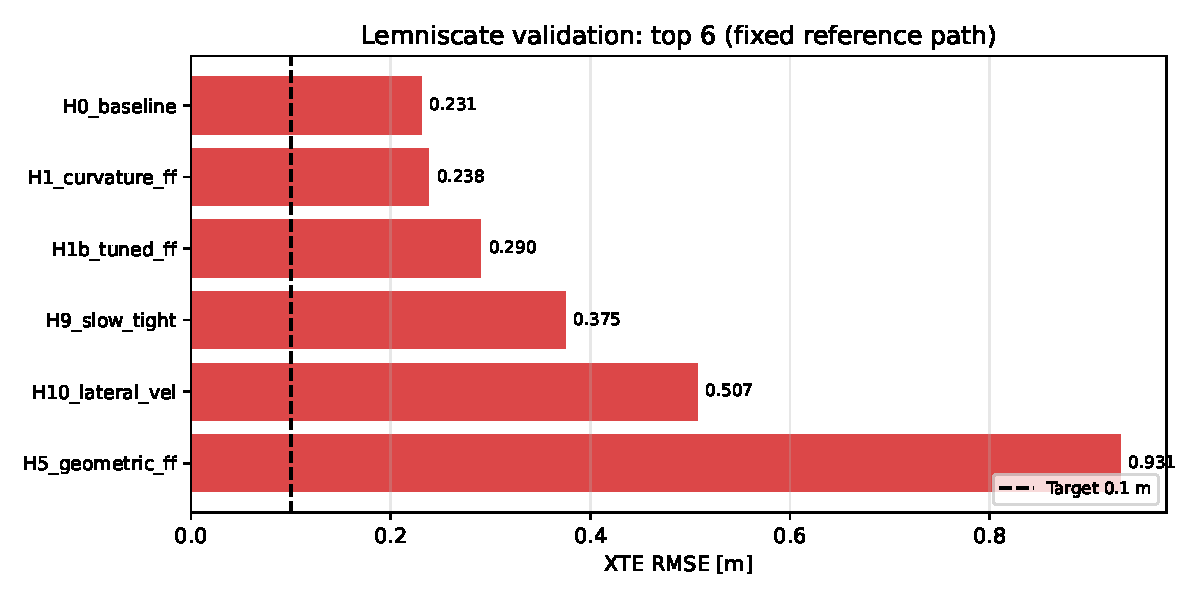
\includegraphics[width=0.88\textwidth]{validation_bar.pdf}
  \caption{Top six approaches: XTE RMSE on the fixed lemniscate reference
           (\texttt{lemniscate\_validation}). Dashed line: \SI{0.1}{\meter} target.}
  \label{fig:val_bar}
\end{figure}

\begin{figure}[H]
  \centering
  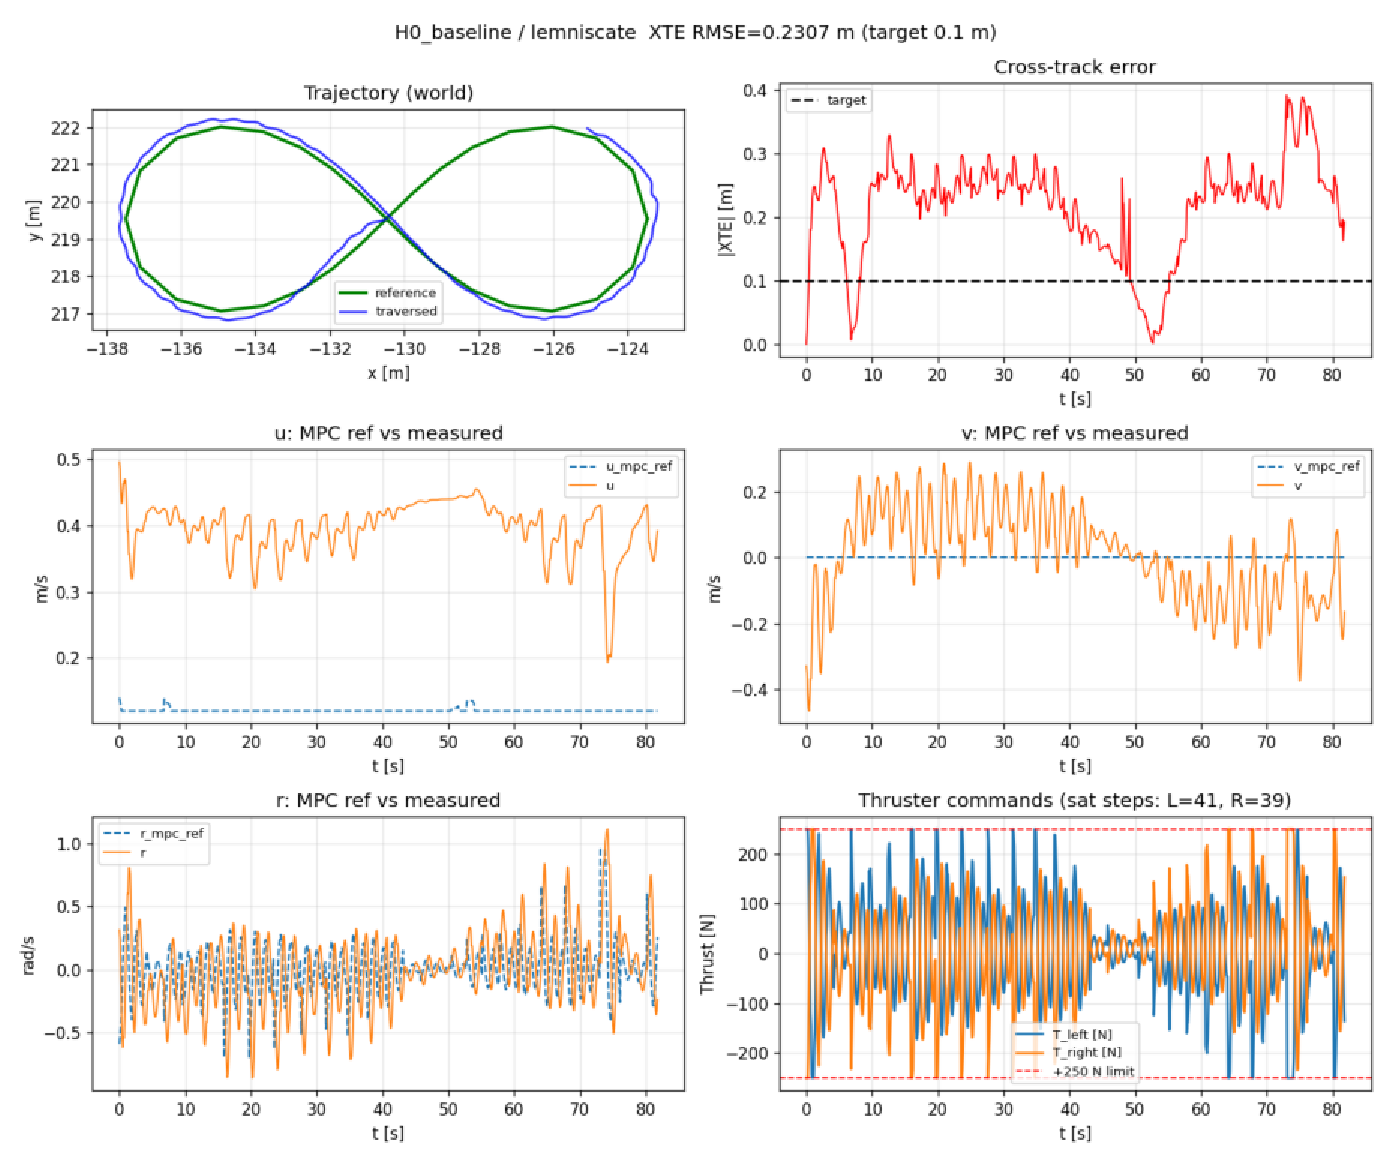
\includegraphics[width=\textwidth]{best_H0_baseline.pdf}
  \caption{Best approach H0\_baseline on the fixed lemniscate: trajectory, XTE,
           velocity MPC tracking ($u,v,r$ vs.\ \texttt{nu\_horizon[0]}), and thruster
           commands with saturation limits ($\pm$\SI{250}{\newton}).}
  \label{fig:best}
\end{figure}

\begin{figure}[H]
  \centering
  \begin{subfigure}[t]{0.48\textwidth}
    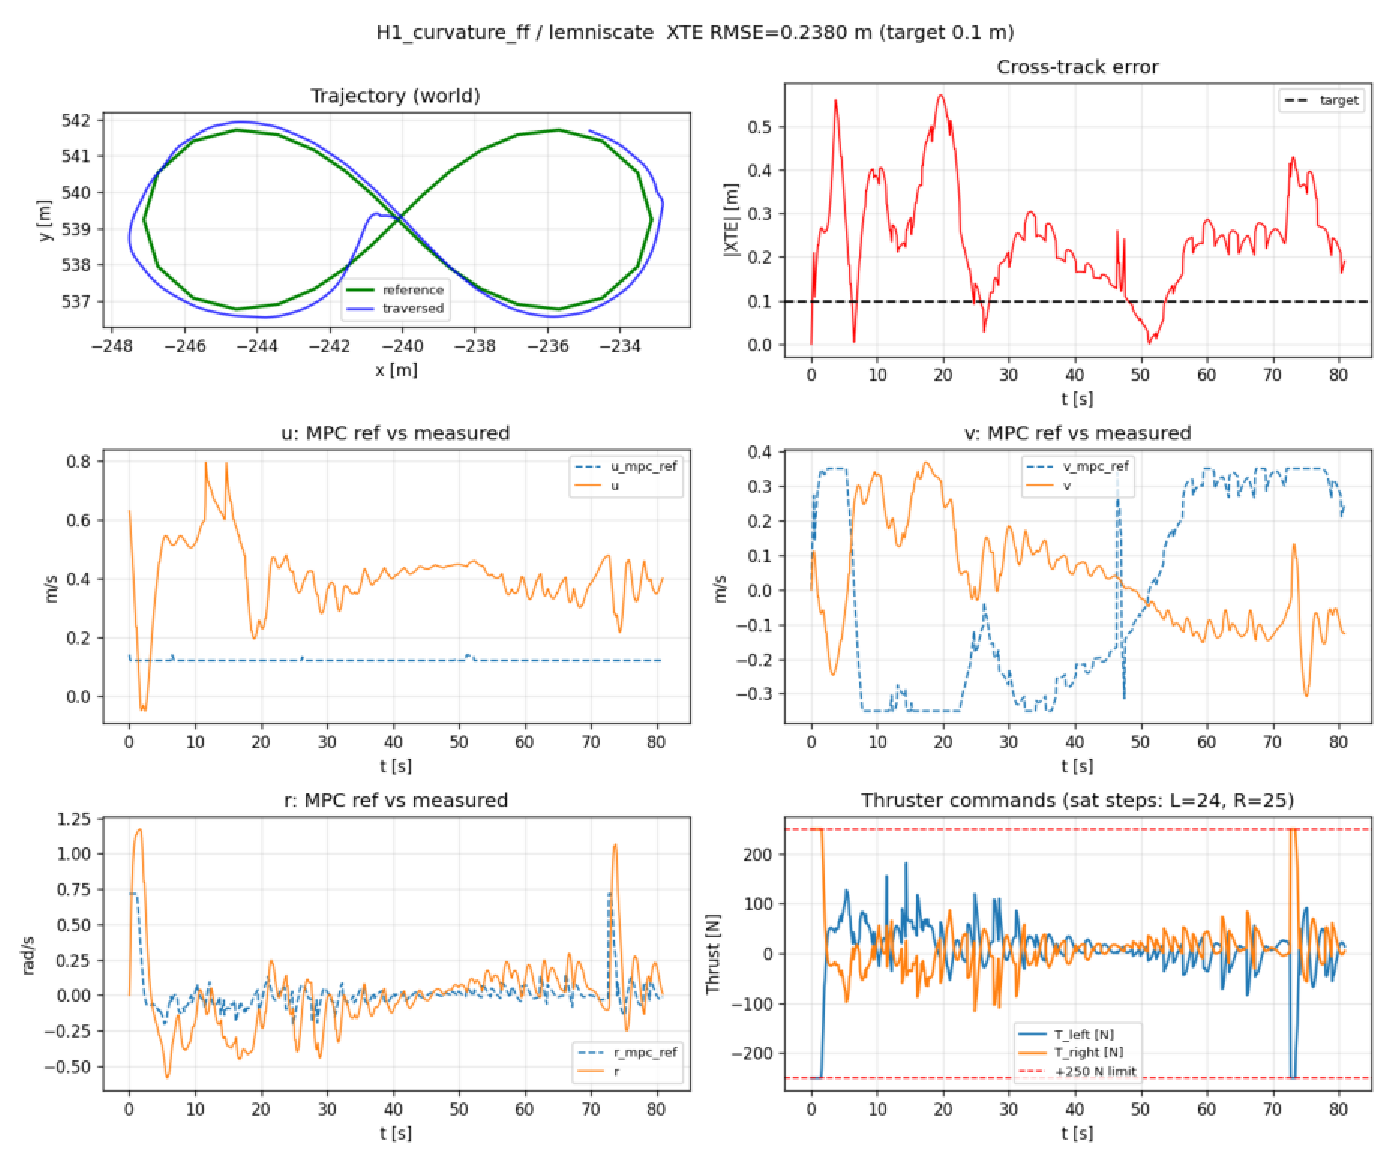
\includegraphics[width=\textwidth]{diag_H1_curvature_ff.pdf}
    \caption{H1\_curvature\_ff (rank 2)}
  \end{subfigure}\hfill
  \begin{subfigure}[t]{0.48\textwidth}
    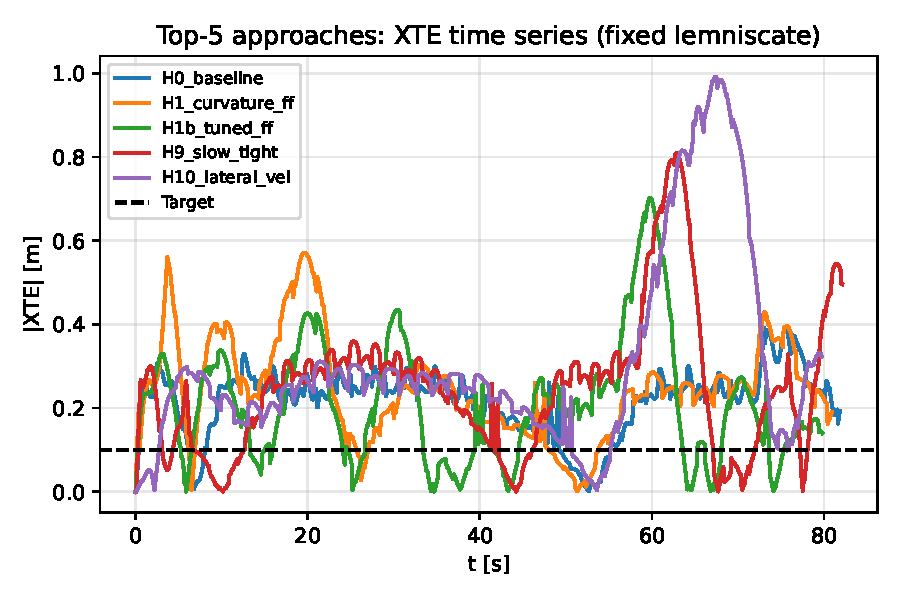
\includegraphics[width=\textwidth]{xte_top6.pdf}
    \caption{Top-5 XTE time series (H5 omitted from top-6)}
  \end{subfigure}
  \caption{Runner-up diagnostics and cross-approach XTE comparison.}
  \label{fig:compare}
\end{figure}

\textbf{Key findings:}
\begin{itemize}[noitemsep]
  \item \textbf{Winner}: H0\_baseline --- \texttt{baseline\_ilos\_velocity} + velocity MPC,
        RMSE \textbf{\SI{0.231}{\meter}} (closest to target among all fifteen approaches).
  \item \textbf{Runner-up}: H1\_curvature\_ff at \SI{0.238}{\meter}; H1b tuned FF at
        \SI{0.290}{\meter}.
  \item \textbf{H9 slow tight}: \SI{0.375}{\meter} on the correct reference
        (previously \SI{0.109}{\meter} on a path corrupted by small Dubins step size).
  \item \textbf{Diagnostics}: extended logging shows MPC tracks $\nu^{\mathrm{ref}}_{0}$ while
        guidance scalars (\texttt{u\_cmd}) can differ; thruster saturation is visible on tight
        curve segments.
  \item \textbf{Target}: none of the fifteen approaches met \SI{0.1}{\meter}.
\end{itemize}

%==============================================================================
\section{Discussion}
\label{sec:discussion}

\subsection{Why velocity MPC + curvature FF succeeded}

The top stack separates \textbf{feasible} inner-loop tracking ($[u,v,r]$ via OSQP) from
\textbf{geometric} outer-loop planning (ILOS + $r=u\kappa$ preview). On this validation run the
conservative H0 baseline edged out curvature-FF variants; H1b's BO-tuned $Q_r$ and
$\kappa$ feedforward did not improve over plain ILOS once the reference path was corrected.
Reduced cruise speed (H9) alone was insufficient.

\subsection{Why lower-ranked approaches failed after BO}

\textbf{Spatial MPC (H11, 122\,m):} path-index jumps on closed curves, large $Q_{xy}$ on an
underactuated plant, and zero $r_{\mathrm{ref}}$ in the spatial preview caused runaway thrust.

\textbf{SMC, Frenet, backstepping, contouring (H12--H16):} aggressive lateral and heading
gains produced oscillation; BO trial minima were not reproducible on validation.

\textbf{Stanley, pure pursuit (H2, H8):} unsuitable for closed lemniscate without structural
changes (lookahead / monotonic arc-length indexing).

\subsection{Diagnostic logging}

\texttt{log.csv} records measured $[u,v,r]$, MPC references
\texttt{u\_mpc\_ref}, \texttt{v\_mpc\_ref}, \texttt{r\_mpc\_ref} (from
\texttt{nu\_horizon[0]}), and pre-saturation thrust in newtons. Per-hypothesis
\texttt{plots.png} overlays MPC refs against measured velocities and marks thruster
saturation at $\pm$\SI{250}{\newton}. Guidance scalars (\texttt{u\_cmd}, \texttt{r\_ref}) are
retained for outer-loop analysis but are not the MPC setpoint.

%==============================================================================
\section{Conclusions}
\label{sec:conclusions}

\begin{enumerate}
  \item \textbf{Best approach}: \textbf{H0\_baseline} ---
        \texttt{baseline\_ilos\_velocity} + velocity MPC (OSQP);
        validation RMSE \textbf{\SI{0.231}{\meter}} on the fixed lemniscate reference.
  \item \textbf{Goal}: RMSE $< \SI{0.1}{\meter}$ not achieved; best margin $\approx$\SI{0.131}{\meter}.
  \item \textbf{Reference path matters}: rankings changed substantially once all approaches
        shared the same 77-point figure-8; Dubins step size must not be BO-tuned on closed curves.
  \item \textbf{Not recommended without redesign}: spatial MPC, pure pursuit, contouring/backstepping
        on closed tight curves in this sim stack.
\end{enumerate}

%==============================================================================
\section{Future Work}
\label{sec:future}

\begin{itemize}
  \item \textbf{Contouring / Frenet NMPC}: penalize $e_d, \dot{e}_d$ with arc-length state.
  \item \textbf{Spatial MPC v2}: monotonic arc-length index, $r_{\mathrm{ref}}=u\kappa$ preview.
  \item \textbf{Hybrid}: retain H9 outer loop; add light position feedback in cost.
  \item \textbf{Validation}: multiple Gazebo seeds per BO winner; report mean $\pm$ std.
\end{itemize}

%==============================================================================
\appendix
\section{Reproduction}
\label{app:repro}

\begin{verbatim}
cd molo_wpt_follower/mpc
python3 experiments/tune_lemniscate.py --n-calls 28
python3 experiments/run_lemniscate_validation.py
python3 experiments/plot_results.py experiments/results/lemniscate_validation --validation
python3 report/generate_figures.py
cd report && make pdf
\end{verbatim}

BO configs: \texttt{experiments/results/tune\_lemniscate\_full/}\\
Validation: \texttt{experiments/results/lemniscate\_validation/}

\section{Hypothesis registry}
Full statements in \texttt{experiments/hypotheses.yaml} and
\texttt{experiments/approaches.yaml}.

\begin{thebibliography}{9}
\bibitem{osqp}
P.~Stellato, G.~Banjac, G.~Goulart, A.~Bemporad, and S.~Boyd,
``OSQP: an operator splitting solver for quadratic programs,''
\emph{Mathematical Programming Computation}, 2020.
\end{thebibliography}

\end{document}
